\chapter{Performance} \label{sec: performance}
%% TODO: maybe think about renaming this chapter into something else, because we here not only talk about performance but also introduce all training/architecture modifications

Models suitable for real-life deployment should be not only fast but also accurate. Definition of "accurate" differs in literature. In this paper we use top-1 classification accuracy on imagenet as proxy for model performance on down-stream tasks, see Section \ref{subsec: imagenet} for detailed discussion. 
The performance of a vision model is a product of the architecture, training methods and regularization. \cite{lee2020_compounding_improvements}. 
Since the introduction of AlexNet \cite{krizhevsky2012_imagenet_alexnet}, many studies emphasizes was on modifying model architectures through new blocks (cite Inception), new architectural choices (cite ResNet ), new rules for scaling models \cite{tan2019_efficientnet} or novel types of regularization. \cite{zhang2017_mixup} \cite{yun2019_cutmix}
% тут можно ещё подробнее написать кто что предлагает
In contrast to these studies focusing on designing new network architecture, works like \cite{he2019_bag_of_tricks} follow different approach to improve model performance. They noted that performance can be improved not only through changes in the model structure, but also through other aspects of network training such as data preprocessing, augmentations, regularization techniques and parameter initialization (cite NFNet). They also demonstrate that these minor “tricks” play a major part in boosting model performance when applied in combination. This improvements are highly significant because it could bring as much performance improvement as a novel network design does. For example \cite{he2019_bag_of_tricks} shows that top-1 validation accuracy of vanilla ResNet-50 could be improved from 75.3\% to 79.2\% with changes in training procedure alone. 

% As a result of using these tricks, ILSVRC2012 top-1 validation ac- curacy of ResNet-50 improved from 75.3\% to 79.29\% and MobileNet improved from 69.03\% to 71.90\%. This improvement is highly significant because it shows as much performance improvement as a novel network design does. 

There is another issue, rarely mentioned in papers. Novel architectures quite often are introduced simultaneously with other important, but less emphasized changes in the details of training methodology and hyperparameters, most refinements are either briefly mentioned as implementation details or only visible in source code. Additionally novel architectures obtained with modern training strategies are sometimes compared to older architectures with outdated training methodology. This systematic error makes comparing new architectures confusing and makes it much more difficult for practitioners to select good-performing architectures. 

% выше последнее предложение как-то не очень хорошо написано конечно 

This work carefully explores current CNN-related techniques for image classification which could be assembled together, and separates then into training / regularization techniques and architectural changes. The first one being non-intrusive, model-agnostic changes capable of boosting almost any existing convolutional deep learning model. And the second one being modifications of architecture, which greatly affect performance with minor impact on model throughput. 



\section{Preliminaries} \label{sec: preliminaries}
For better understanding we first describe default experimental setup for training ResNet50 model along with it's architecture and description of used dataset and metrics. 

\paragraph{Dataset} \label{subsec: imagenet}

% эту часть нужно перенести в главу 4 про эксперименты
% (сюда можно дописать еще общих слов из \cite{beyer2020_are_we_done}) для объема

Imagenet Large Scale Vision Recognition Challenge also known as ILSVRC2012 or simply Imagenet has been a central testbed of research in artificial perception for almost a decade and it's scale and difficulty have highlighted landmark achievements in machine learning. It has 1.3 millions training images divided into 1000 classes. Validation dataset consist of 50 thousand images, equally balanced between same 1000 classes. ILSVRC2012 is the most used dataset in computer vision. % \cite{something related}
In recent years with models becoming larger and demanding more and more data, it became a de-facto standard benchmark for any new architecture. Since the breakthrough of AlexNet improving convolutional neural networks lead to improvements in other fields of computer vision. Typically researchers optimize models on classification problems using ImageNet \cite{deng2009_imagenet} as proxy. It has been shown \cite{he2019_bag_of_tricks} \cite{kornblith2019_better} than improvements from Imagenet increase transfer learning performance in other domains, for example object detection and semantic segmentation.


In this paper we will use top-1 classification accuracy on the ILSVRC2012 validation dataset as metric of model performance. It shows the percentage of correctly classified images and has a very strong correlation of $r=0.96$ \cite{kornblith2019_better} between ImageNet accuracy and transfer learning accuracy, which makes it a well suitable metric.

\paragraph{Baseline Training Procedure} \label{subsec: baseline_training}
This section introduces training hyperparameters for Imagenet following \cite{he2016identity_resnetv2} paper. The preprocessing differs between training and validation. Steps performed during training:
\begin{itemize}
    \item Sample a random image and decode it into 32-bit floating point raw pixel values in [0, 255].
    \item Randomly crop a rectangular region whose aspect ratio is randomly sampled in [3/4, 4/3] and area randomly sampled in [8\%, 100\%], then resize the cropped region into a 224-by-224 square image.
    \item Flip horizontally with 0.5 probability.
    \item Scale hue, saturation, and brightness with coefficients uniformly drawn from [0.6, 1.4].
    \item Add PCA noise with a coefficient sampled from a normal distribution N (0, 0.1)
    \item Normalize RGB channels separately by subtracting $(123.7, 116.8, 103.9)$ and dividing by $(58.4, 57.1, 57.4)$, respectively.
\end{itemize}

During validation random augmentations is not used. Steps performed for validation are:

\begin{itemize}
  \item Image's shortest size is resized to 256 pixels with aspect ration remaining the same
  \item A center 224-by-224 region of the image is cropped
  \item RGB channels are normalized similar to training
\end{itemize}

% TODO: rewrite this copy-pasted piece below
The weights of both convolutional and fully-connected layers are initialized with the Xavier algorithm [6]. In particular, we set the parameter to random values uniformly drawn from $[−a, a]$, where $ a = \sqrt{6 / (d_{in} + d_{out})} $ Here $d_{in}$ and $d_{out}$ are the input and output channel sizes, respectively. All biases are initialized to 0. For batch normalization layers, $\gamma$ vectors are initialized to 1 and $\beta$ vectors to 0.
Stochastic Gradient Descent (SGD) is used for training. Model is trained for 100 epochs a batch size of 256 per GPU. The learning rate is initialized to 0.1 and divided by 10 at the 30th, 60th, and 90th epochs. % TODO \cite{something for SGD}

% TODO: maybe add more details about drawbacks of current architecture 
This training pipeline described above was de-facto standard for researchers of Imagenet, despite it's several drawbacks discussed later. 

\paragraph{Baseline Model Architecture}
This section briefly presents the ResNet architecture, especially its modules. For detailed information please refer to \cite{he2016deep_resnetv1}


\begin{figure}[h!]
    \centering
    \label{fig: resnet-a}
    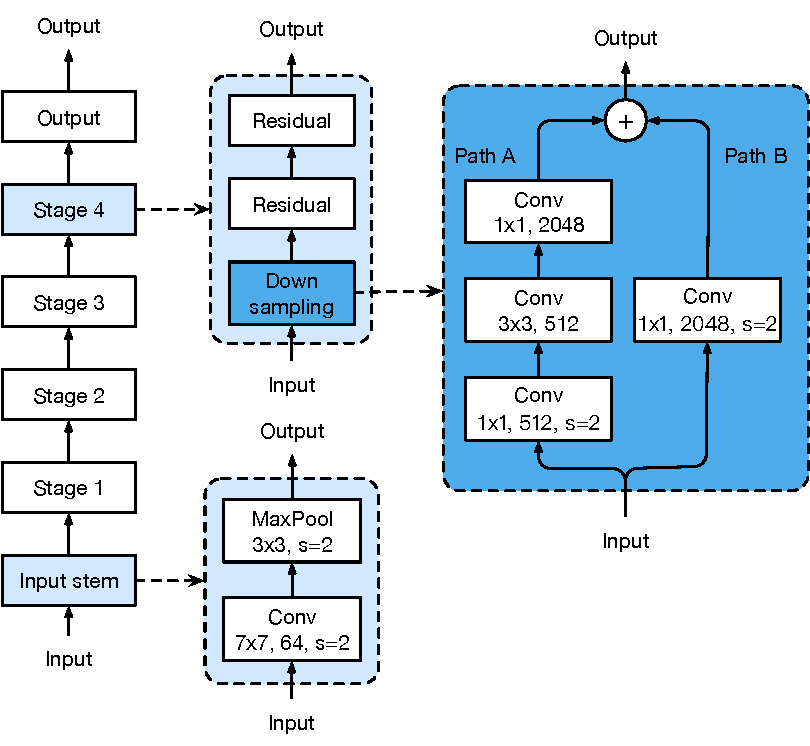
\includegraphics[width=0.5\textwidth]{images/resnet-a.pdf}
    \caption{The architecture of ResNet-50. The convolution kernel size, output channel size and stride size (default is 1) are illustrated, similar for pooling layers}
  \end{figure}


% below is again a large copy-paste
A ResNet network consists of an input stem, four subsequent stages and a final output layer, which is illustrated in Figure \ref{fig: resnet-a}. The input stem has a $7 \times 7$ convolution with an output channel of 64 and a stride of 2, followed by a $3 \times 3$ max pooling layer also with a stride of 2. The input stem reduces the input width and height by 4 times and increases its channel size to 64. 
Starting from stage 2, each stage begins with a downsampling block, which is then followed by several residual blocks. In the downsampling block, there are path A and path B. Path A has three convolutions, whose kernel sizes are $1 \times 1$, $3 \times 3$ and $1 \times 1$, respectively. The first convolution has a stride of 2 to halve the input width and height, and the last convolution’s output channel is 4 times larger than the previous two, which is called the bottleneck structure. Path B uses a 1×1 convolution with a stride of 2 to transform the input shape to be the output shape of path A, so we can sum outputs of both paths to obtain the output of the downsampling block. A residual block is similar to a downsampling block except for only using convolutions with a stride of 1.
One can vary the number of residual blocks in each stage to obtain different ResNet models, such as ResNet-50 and ResNet-152, where the number presents the number of convolutional layers in the network.


% 
% 2.1. Baseline Training Procedure
% We follow a widely used implementation [8] of ResNet as our baseline. The preprocessing pipelines between train- ing and validation are different. During training, we per- form the following steps one-by-one:
% 1. Randomly sample an image and decode it into 32-bit floating point raw pixel values in [0, 255].
% 2. Randomlycroparectangularregionwhoseaspectratio is randomly sampled in [3/4, 4/3] and area randomly sampled in [8%, 100%], then resize the cropped region into a 224-by-224 square image.
% 3. Flip horizontally with 0.5 probability.
% 4. Scale hue, saturation, and brightness with coefficients
% uniformly drawn from [0.6, 1.4].
% 5. Add PCA noise with a coefficient sampled from a nor-
% mal distribution N (0, 0.1).
% 6. Normalize RGB channels by subtracting 123.68, 116.779, 103.939 and dividing by 58.393, 57.12, 57.375, respectively.
% During validation, we resize each image’s shorter edge to 256 pixels while keeping its aspect ratio. Next, we crop out the 224-by-224 region in the center and normalize RGB channels similar to training. We do not perform any random augmentations during validation.
% The weights of both convolutional and fully-connected layers are initialized with the Xavier algorithm [6]. In particular, we set the parameter to random values uniformly drawn from [−a, a], where a = 􏰇6/(din + dout ). Here din and dout are the input and output channel sizes, respectively. All biases are initialized to 0. For batch normalization layers, γ vectors are initialized to 1 and β vectors to 0.
% Nesterov Accelerated Gradient (NAG) descent [20] is used for training. Each model is trained for 120 epochs on 8 Nvidia V100 GPUs with a total batch size of 256. The learning rate is initialized to 0.1 and divided by 10 at the 30th, 60th, and 90th epochs.


% тут нужно как-то сказать что в этой главе мы меняем только базовый резнет, а более серьезные изменения, объединяющие выводы главы 2 и 3 представлены в главе 4

\section{Large-batch tricks} \label{sec: large-batch}

% this section is very inspired and mostly copy-pasted from "Bags of Tricks.... "
Modern accelerators allow usage of very large batch-size for mini-batch SGD optimization to decrease communication costs, increase parallelism and speedup the training. However, large batch size may slowdown the speed convergence, for the same number of steps, models trained with larger batch size result in slightly lower validation accuracy compared to the models trained with small batch-sizes. This has been noticed before and multiple heuristic has been proposed ...

cite [7]: accurate large minibatch SGD training imagenet in 1 hour
cite [14]: Highly scalable deep-learning training system with mixed precision. training imagenet in four minutes

to solve this issue. The following paragraphs describe four popular heuristics used to allow scaling the batch size up. 

\paragraph{Learning rate warmup.}
Due to random initialization of neural networks parameters, at the beginning of training all weighs are far from the final solution and gradients are noisy. Using a large learning rates results in numerical instability and slowdown further training. The solution to this problem is to set learning rate to 0 at the beginning and linearly increase it to initial learning rate during first $m$ batches (typically 5 data epochs). cite [7] cite[9]. For example, if our initial learning rate is $\eta$, then at batch $i, 1 < \leq i \leq m$, the learning rate would be $ i \eta / m$.

\paragraph{Zero $\gamma$.} % this paragraph is fully copy-pasted. TODO: rewrite it
A ResNet network consists of multiple residual blocks, each block consists of several convolutional layers. Given input $x$, assume block $(x)$ is the output for the last layer in the block, this residual block then outputs $x+$ block $(x)$. Note that the last layer of a block could he a batch normalization (BN) layer. The BN layer first standardizes its input, denoted by $\hat{x}$, and then performs a scale transformation $\gamma \hat{x}+\beta .$ Both $\gamma$ and $\beta$ are learnable parameters whose elements are initialized to $1 \mathrm{~s}$ and $0 \mathrm{~s}$, respectively. In the zero $\gamma$ initialization heuristic, we initialize $\gamma=0$ for all BN layers that sit at the end of a residual block. Therefore, all residual blocks just return their inputs, mimics network that has less number of layers and is easier to train at the initial stage.

\paragraph{Linear scaling learning rate.}
In mini-batch SGD, gradient descending is a random process because the examples are randomly selected in each batch. Increasing the batch size does not change the expectation of the stochastic gradient but reduces its variance. In other words, a large batch size reduces the noise in the gradient, so we may increase the learning rate to make a larger progress along the opposite of the gradient direction. Goyal et al. $[7]$ reports that linearly increasing the learning rate with the batch size works empirically for ResNet-50 training. In particular, if we follow He et al. [9] to choose $0.1$ as the initial learning rate for batch size 256, then when changing to a larger batch size $b$, we will increase the initial learning rate to $0.1 \times b / 256 .$

\paragraph{No bias decay.}
The weight decay is a popular technique used to prevent overfitting. It's usually applied to all parameters in the model, including weights, biases, $\gamma$ and $\beta$ in BN layer. It's similar to an L2 regularization which drives all values towards $0$. However, in order to prevent overfitting it's enough to apply weight decay only to weights of convolutional and fully-connected layers cite[14]. The no bias decay heuristic removes regularization from bias terms in convolutions and parameters of BN layers, increasing the model expressiveness while still helping to counter overfit.  


\section{Training Refinements}

Here we present regularization and data augmentation strategies routinely used in state-of-the art classification models \cite{lin2020neural_genet} \cite{tan2019_efficientnet} \cite{tan2021_efficientnetv2}

\paragraph{Data Augmentation}
Default augmentations used in Imagenet training described in Section \ref{subsec: baseline_training} are quite weak to match up the capacity of modern CNNs. Many better augmentations strategies has been proposed to bring diversity during training. Two most popular being: 

\begin{itemize}
    \item AutoAugment \cite{cubuk2018_autoaugment} which learns augmentation strategies from data. It uses reinforcement learning to select a sequence of image augmentation operations with the best accuracy by searching a discrete search space of their probability of application and magnitude.
    \item RanAug \cite{cubuk2020_randaugment} also applies reinforcement learning, but to a significantly reduced search space in order to find sequence of random image transformations (e.g. translate, shear, color distortions) for each image
\end{itemize}

\begin{figure}[h!]
    \caption{One of the successful policies on ImageNet. As described in the text, most of the policies found on ImageNet used color-based transformations.}
    \label{fig: randaug}
    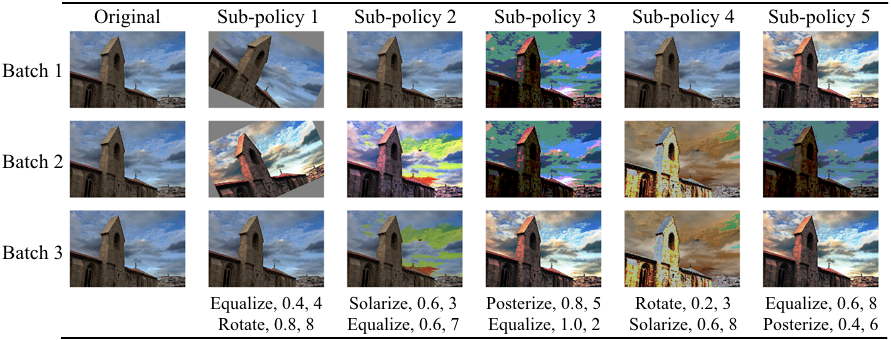
\includegraphics[width=0.5\textwidth]{images/randaug_policy.png}
  \end{figure}

Both of this policies use extensive amount of augmentations in the color domain combined with hard affine transformations like rotation and shear. Example of augmentations could be seen on Figure \ref{fig: randaug}
From out experiments we found that RandAug slightly outperforms AutoAugment, so we use the former later in the text. The exact definition of RandAug augmentation strategy on Imagenet could be found in Appendix. 
% TODO: add RandAug strategy to appendix.


\paragraph{MixUp and CutMix}


Mixup \cite{zhang2017_mixup} and CutMix \cite{yun2019_cutmix} are two recently proposed augmentation and regularization strategies. They both create new examples by interpolating two examples of the training set. Neural networks are known to memorize training data rather than generalize from the data \cite{zhang2016_understanding_deep}. As a result, the neural network produces unexpected outputs when it encounters data which are different from the distribution of the training set. Mixup/CutMix mitigates the problem by showing the neural network interpolated examples, and this helps to fill up the empty feature space of the training dataset.

% TODO: fix this table, remove cutout from it
% original cutmix table. I don't know how to increase it so using the version below for now. But this one looks better IMHO
% \begin{table}[h!]
%   \centering
%   \small
%   \tabcolsep=0.07cm
%   \begin{tabular}{@{}ccccc@{}}
%   & Original  &  Mixup \cite{zhang2017_mixup} & CutMix \cite{yun2019_cutmix}\\
%   \multirow{4}{*}{Image} &  \multirow{4}{*}{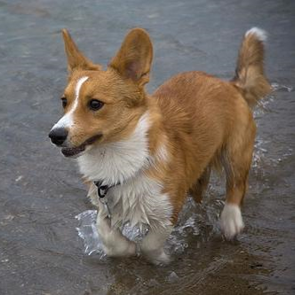
\includegraphics[width=0.10\linewidth]{images/dog.png}}
%   &  \multirow{4}{*}{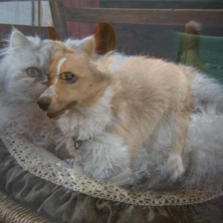
\includegraphics[width=0.10\linewidth]{images/dog_mixup.png}}
%   &  \multirow{4}{*}{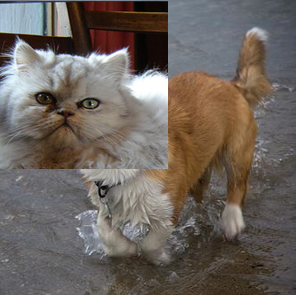
\includegraphics[width=0.10\linewidth]{images/dog_cutmix.png}} \\ 
%   & & & \\ 
%   & & & \\
%   & & & \\ \midrule
%   %
%   \multirow{2}{*}{Label} 
%   &\multirow{2}{*}{Dog 1.0}
%   &\multirow{2}{*}{\begin{tabular}[c]{@{}c@{}}Dog 0.5\\ Cat 0.5\end{tabular}}
%   &\multirow{2}{*}{\begin{tabular}[c]{@{}c@{}}Dog 0.6\\ Cat 0.4\end{tabular}} \\ 
%     & & & \\  \toprule

%   \end{tabular}
%   \caption{Example of Mixup/CutMix augmentations}
%   \label{tab:cutmix}
%   \end{table}


  \begin{figure}[h!]
    \centering
    \subfloat[][Original \\ Dog 1.0]{
      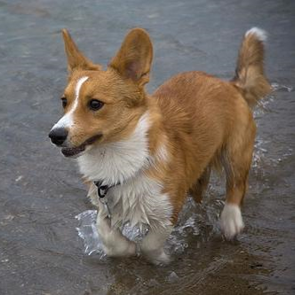
\includegraphics[scale=.55]{images/dog.png}
    }\hfill%
    \subfloat[][Mixup \\ Dog 0.5 Cat 0.5]{
      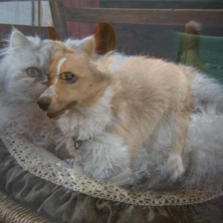
\includegraphics[scale=.55]{images/dog_mixup.png}
    }\hfill%
    \subfloat[][Cutmix \\ Dog 0.6 Cat 0.4]{
      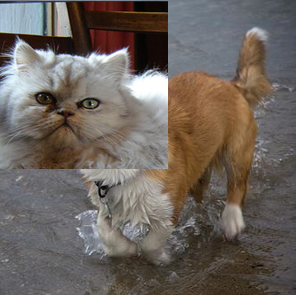
\includegraphics[scale=.55]{images/dog_cutmix.png}
    }
    \caption{Example of Mixup/CutMix augmentations. Label for each image during training is shown in sub-captions.}
    \label{fig:cutmix}

  \end{figure}

% below is copy-paste
CutMix shares similarity with Mixup which mixes two samples by interpolating both the image and labels. While certainly improving classification performance, Mixup samples tend to be unnatural and locally ambiguous, and therefore confuses the model. CutMix overcomes the problem by replacing the image region with a patch from another training image, producing a more natural results as could be seen in Figure \ref{tab:cutmix}

Mixup/CutMix has two types of implementation. The first type uses two mini batches to create a mixed mini batch. this type of implementation is suggested in the original paper \cite{zhang2017_mixup}. The second type uses a single mini batch to create the mixed mini batch by mixing the single mini batch with a shuffled clone of itself. The second type of implementation uses less CPU resources because only one mini batch needs to be preprocessed to create one mixed mini batch. However, experiments show that the second type of implementation reduces top-1 accuracy \cite{lee2020_compounding_improvements}. Therefore, in later experiments, we use the first type of implementation. We set the Mixup hyperparameter $\alpha$ to 0.2 and Cutmix alpha to 1. 


% TODO: вставить больше формул про то, что такое CutMix https://sh-tsang.medium.com/paper-cutmix-regularization-strategy-to-train-strong-classifiers-with-localizable-features-5527e29c4890


\paragraph{Label Smoothing}

Label smoothing is a regularization technique widely used in many state-of-the-art models, including image classification, language translation and speech recognition. (TODO: cite smth here. examples are already in bib). The idea of label smoothing is that generalization of neural networks often could be significantly improved by adding the uniform distribution over labels to hard targets. Such smoothing prevents the model from predicting the labels to confidently improving the calibration of the model.  Mathematical description of label smoothing is as follows. For classification problem with $N$ classes let $z_i$ be the predicted score for class $i$. This scores are normalized using softmax to obtain predicted probabilities $p_i$ of each class. $p_i = \frac{exp(z_i)}{\sum_{j=1}^N exp(z_j)} $. During training with hard targets we minimize the expected negative cross-entropy loss $H(y, p) = \sum_{i=1}^N -y_k log(p_k)$, where $y_k$ is $1$ for correct class and $0$ for the rest. During training with label-smoothed targets with parameter $\alpha$ we minimize negative cross-entropy loss between the networks probabilities $p_k$ and modified targets  $y_l^{LS}$, where $y_l^{LS} = y_k (1 - \alpha ) + \alpha / N$. It can be shown \cite{he2019_bag_of_tricks} that label smoothing target encourages finite outputs for output layer and thus avoids over-confidence.


\paragraph{Stochastic Depth}

Stochastic depth \cite{huang2016_stochastic_depth} randomly drops each layer (with residual connection around it), effectively changing number of layers in the network. Drop probability is linearly increased from $0$ at the beginning to some value $p_d$ at the end.

\paragraph{Exponential moving average (EMA) of weights}

Exponential moving average of model weights \cite{izmailov2018_averaging_swa_ema} is a technique that leads to a better generalization that conventional training. As was noticed in \cite{garipov2018_loss_surfaces} that flat optimiums lead to better generalization and indicate less overfitting, it could be achieved by simultaneously computing a second set of weights during training and using this weights for final validation. Given decay rate $\alpha$ and network parameters at each step $\theta_{1 \cdots T}$ the corresponding EMA weights are calculated as follows: $\theta_{t}^{EMA} = \alpha \theta_{t-1}^{EMA} + (1 - \alpha) \theta_{t} $. Typically $\alpha$ is set very close to zero, for example 0.999 \cite{tan2021_efficientnetv2} 

\paragraph{Cosine Learning Rate Decay}

% TODO: below is a copy-paste. need to rewrite
Learning rate adjustment is crucial to the training. After the learning rate warmup described in Section \ref{sec: large-batch}, we typically steadily decrease the value from the initial learn- ing rate. The widely used strategy is exponentially decaying the learning rate. He et al. [9] decreases rate at 0.1 for ev- ery 30 epochs, we call it “step decay”. Szegedy et al. [26] decreases rate at 0.94 for every two epochs.
In contrast to it, Loshchilov et al. [18] propose a cosine annealing strategy. An simplified version is decreasing the learning rate from the initial value to 0 by following the cosine function. Assume the total number of batches is T (the warmup stage is ignored), then at batch t, the learning rate ηt is computed as:
$\eta_{t}=\frac{1}{2}\left(1+\cos \left(\frac{t \pi}{T}\right)\right) \eta$, where $\eta$ is the initial learning rate. We call this scheduling as “cosine” decay.

The comparison between step decay and cosine decay are illustrated in Figure \ref{fig:learning-rate-curve}. As can be seen, the cosine decay decreases the learning rate slowly at the beginning, and then becomes almost linear decreasing in the middle, and slows down again at the end. Compared to the step decay, the cosine decay starts to decay the learning since the beginning but remains large until step decay reduces the learning rate by 10x, which potentially improves the training progress.
% end of copy-paste

\begin{figure}[t!]
  \centering
  \subfloat[Learning Rate Schedule\label{fig:lr-schedule}]{%
    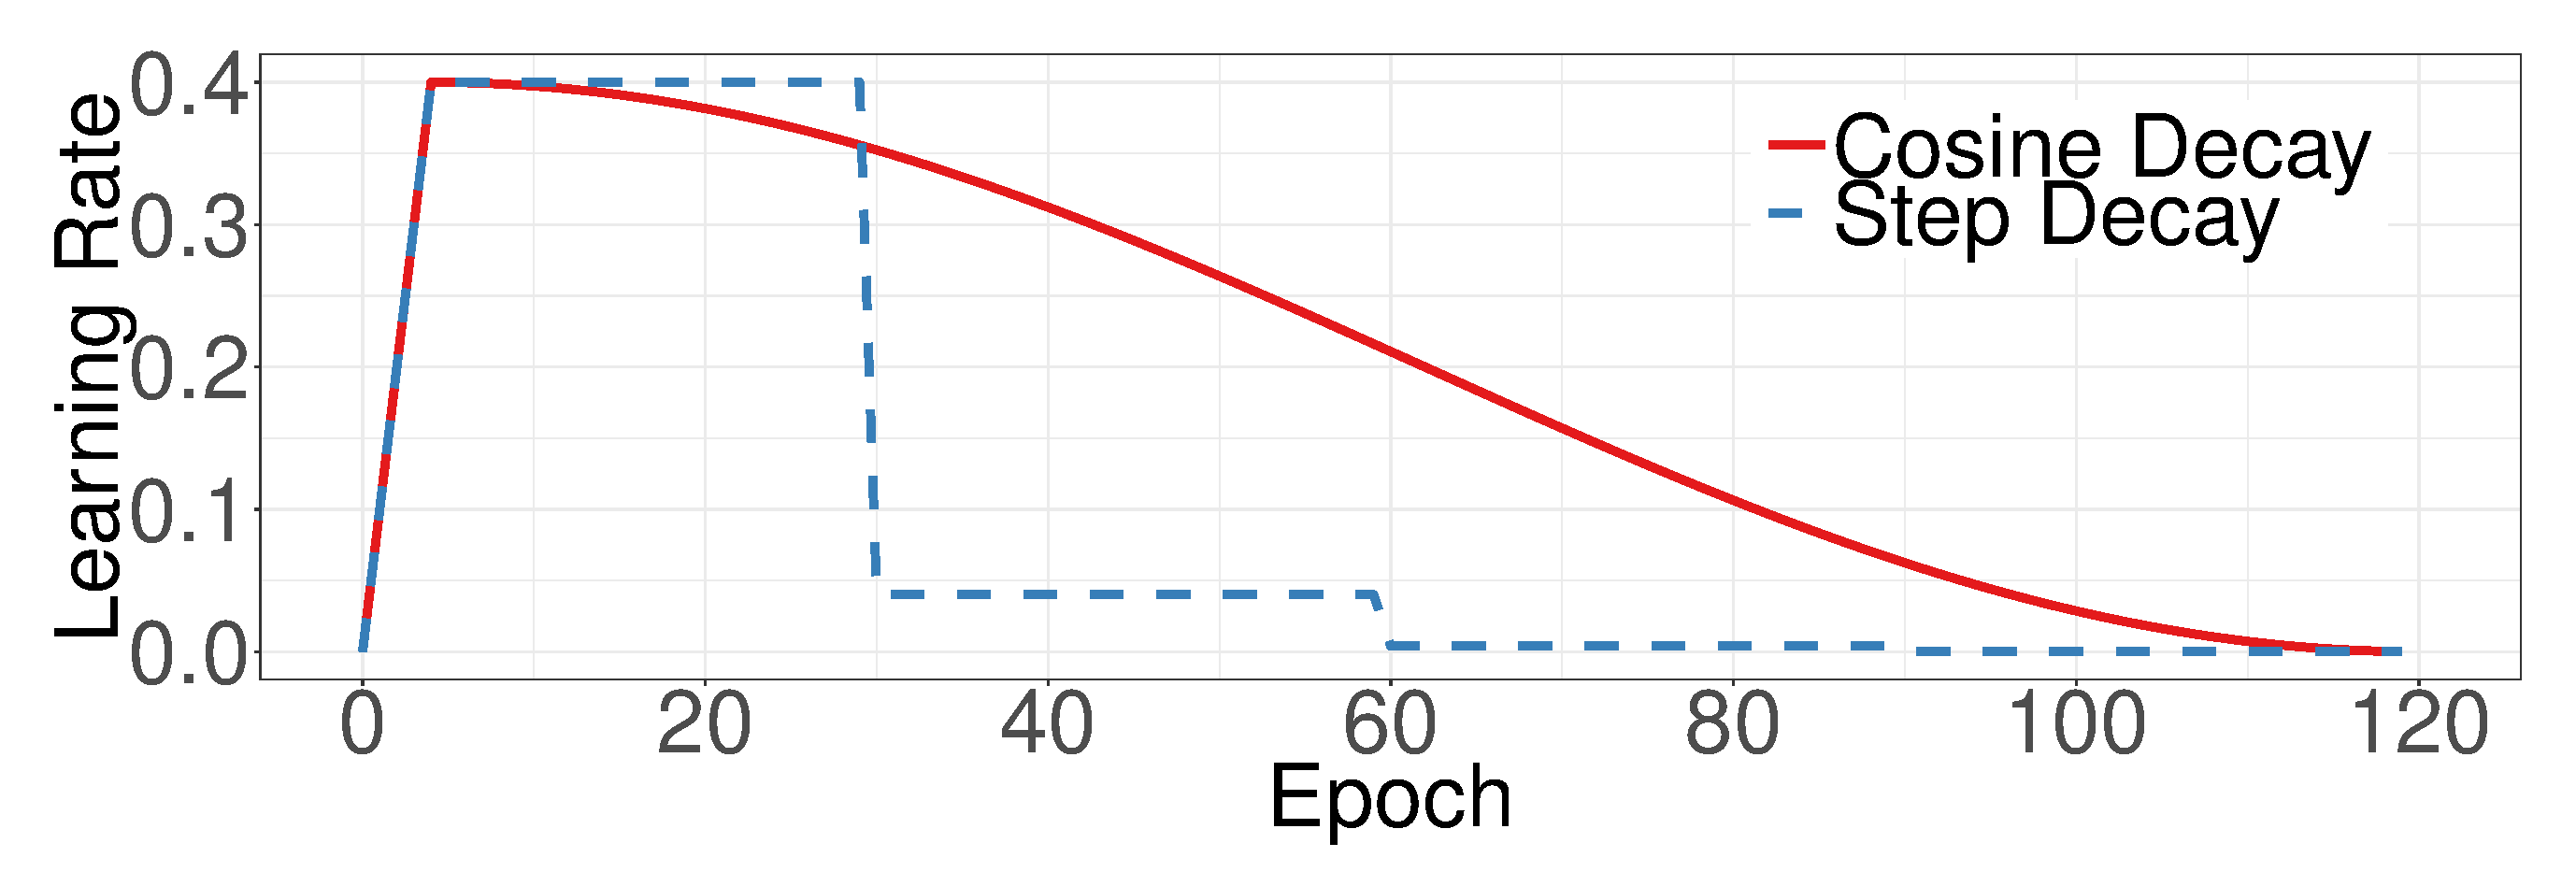
\includegraphics[width=0.5\textwidth]{images/LearningRate-Warmup-thick.pdf}
    } %\vfill%
  \subfloat[Validation Accuracy\label{fig:lr-curve}]{%
    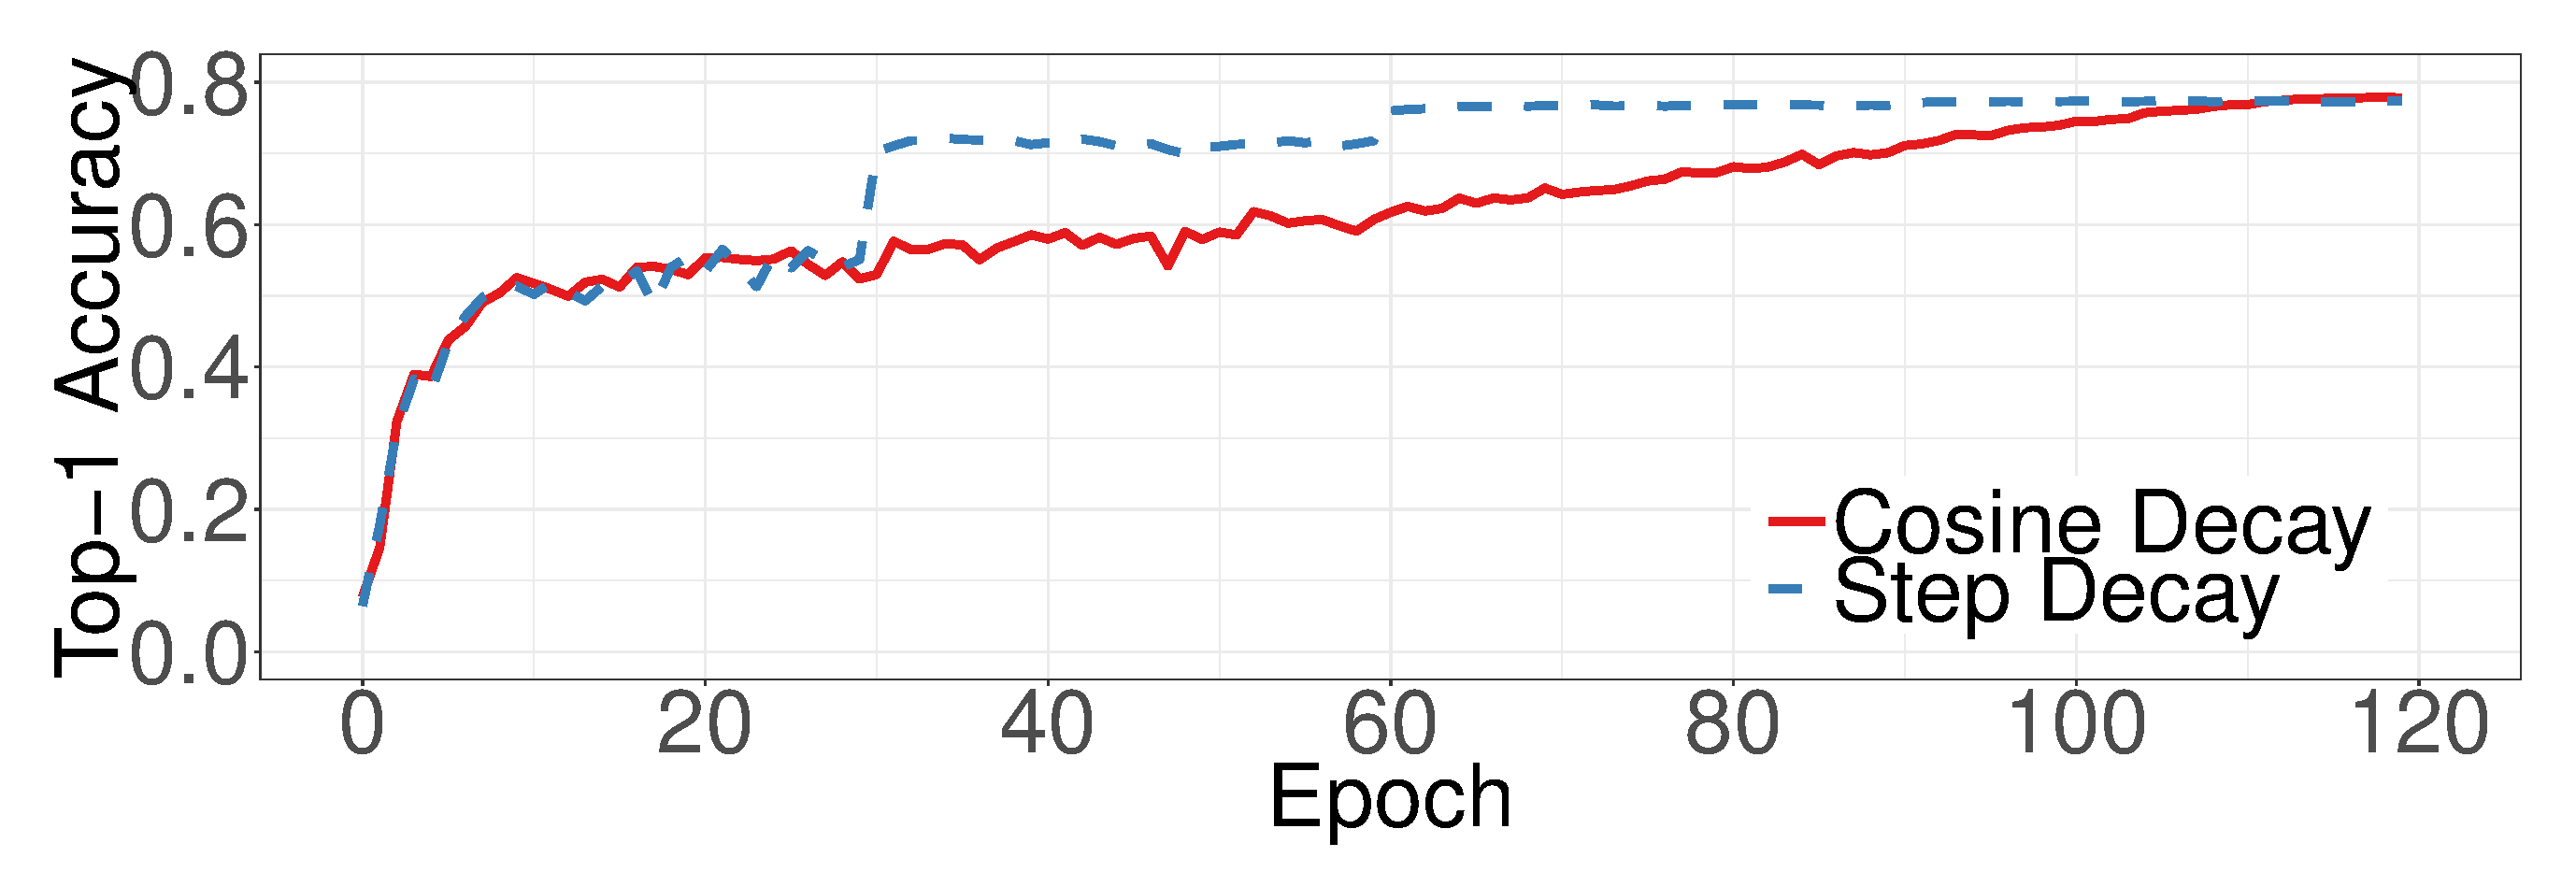
\includegraphics[width=0.5\textwidth]{images/LearningRate-Warmup-curve.pdf}
    }%
  \caption{Visualization of learning rate schedules with warm-up. (a) cosine and step schedules for batch size 1024. (b) Top-1 validation accuracy curve with regard to the two schedules.}
  \label{fig:learning-rate-curve}
\end{figure}







\section{Architecture changes}

Here we present minor adjustments to the model architecture, many of the tweaks presented have very light impact on computational complexity and latency, but often have noticeable effect on the model accuracy. All modifications in this section are applied on top of vanilla ResNet50 model described in Section \ref{sec: preliminaries}.

\subsection{ResNet-B, C, D}
Here we revisit three very common tweaks, which we call ResNet-B, ResNet-C and ResNet-D respectively. This tricks has been first combined in \cite{he2019_bag_of_tricks} and widely used after that \cite{ridnik2021_tresnet} \cite{bello2021_revisiting_resnet}. 

\paragraph{ResNet-B}
First tweak was first introduced in a Torch implementation of the original ResNet model and then was widely adopted by following works [7, 12, 27] (citations from Bag of Tricks). The observation is that convolution in path A on Figure \ref{fig: resnet-a} ignores $3/4$ of the input because it uses a kernel size $1 \times 1$ with a stride of 2. By moving the stride to $3 \times 3$ convolution we can make sure no information is ignored, as shown on Figure \ref{fig:resnet-b}

% ResNet-B. This tweak first appeared in a Torch imple- mentation of ResNet [8] and then adopted by multiple works [7, 12, 27]. It changes the downsampling block of ResNet. The observation is that the convolution in path A ignores three-quarters of the input feature map because it uses a kernel size 1×1 with a stride of 2. ResNet-B switches the strides size of the first two convolutions in path A, as shown in Figure 2a, so no information is ignored. Because the second convolution has a kernel size 3 × 3, the output shape of path A remains unchanged.


\paragraph{ResNet-C}
Second observation is that the computational cost of a convolution is quadratic in respect to the kernel size. First $7 \times 7$ convolution in the network is $5.4$ times more expensive than a $3 \times 3 $ convolution. So replacing it with three $3 \times 3 $ convolutions gives the same receptive field, but requires less computation see Figure \ref{fig:resnet-c}. On practice the overhead for performing 3 separate convolutions makes this variant slightly slower but consistently improves performance \cite{he2019_bag_of_tricks}. 


% This tweak was proposed in Inception-v2 [26] originally, and it can be found on the implementations of other models, such as SENet [12], PSPNet [31], DeepLabV3 [1], and ShuffleNetV2 [21]. The observation is that the computational cost of a convolution is quadratic to the kernel width or height. A 7 × 7 convolution is 5.4 times more expensive than a 3 × 3 convolution. So this tweak replacing the 7 × 7 convolution in the input stem with three conservative 3 × 3 convolutions, which is shown in Figure 2b, with the first and second convolutions have their output channel of 32 and a stride of 2, while the last convolution uses a 64 output channel.

\paragraph{ResNet-D}
Third observation is similar to ResNet-B. In the path B of the downsampling block the $1 \times 1$ convolution also ignores $3/4$ of the input. Adding a $2 \times 2$ average pooling layer before the convolution makes sure nothing is ignored, having a neglitable impact on model latency. This tweak is illustrated on Figure \ref{fig:resnet-d}.

\begin{figure}[t!]
  \centering
  \subfloat[\label{fig:resnet-b}]{
    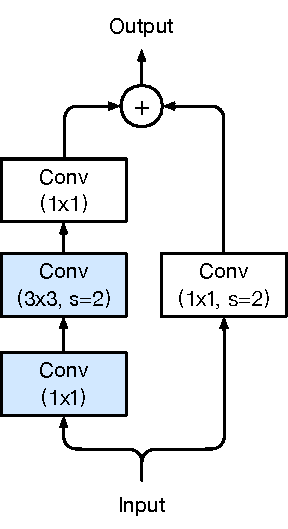
\includegraphics[scale=.55]{images/resnet-b}
  }\hfill%
  \subfloat[\label{fig:resnet-c}]{
    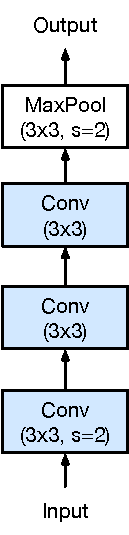
\includegraphics[scale=.55]{images/resnet-c}
  }\hfill%
  \subfloat[\label{fig:resnet-d}]{
    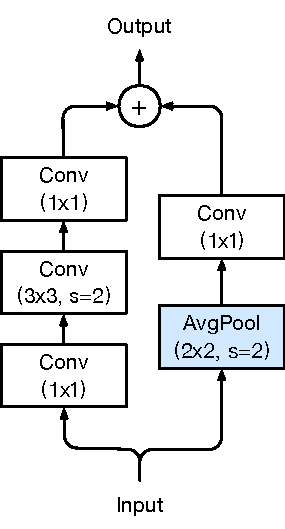
\includegraphics[scale=.55]{images/resnet-d}
  }
  \caption{Three ResNet tweaks. (a) modifies the downsampling block of Resnet. (b) modifies the input stem. (c) again modifies the downsampling block.}
  \label{fig:resnet-tweaks}
\end{figure}


\subsection{Anti-Alias Downsampling (AA)}
% below is copy-paste from Compounding ...
Convolutional networks are vulnerable to small amounts of distortion \cite{xie2020_adversarial}, as small input shifts or translations can cause noticeable change in the output. This contradicts the shift-invariant nature of convolution operation. Such shift-variance is introduced due to commonly used downsampling methods, such as max-pooling and strided convolution. The \cite{zhang2019_making_aa_shift_invariant} proposes Anti-Aliasing downsampling modules as a low-pass filter to improve the shift-equivariance of deep networks. The usual max-pool operation could be viewed as first densely evaluating max operator, followed by naive sub-sampling. By introducing additional blurring operation before sub-sampling we could achieve better anti-aliasing. In the original paper authors propose to AA all downsampling operations present in the model, but on practice \cite{lee2020_compounding_improvements} adding AA with kernel size 3 only after $3 \times 3 $ convolution is enough and gives the best tradeoff between performance improvement and decrease in latency. Based on this results, in the following experiments we apply AA only to strided-convs in the model. 





\subsection{Channel Attention} \label{sec:channel-attn}
Incorporating channel attention mechanism \cite{hu2018_squeeze_SE} \cite{wang2020_eca} into convolutional blocks has shown a great potential in improving the performance of deep convolutional neural networks. % cite  [14, 33, 13, 4, 9, 18, 7]. from ECA paper
Following \cite{hu2018_squeeze_SE} many variants of attention has been proposed, however most existing methods focus on developing sophisticated attention modules, not taking into account model complexity and inference speed. Here we review two most popular methods which don't affect speed too much. See Figure \ref{fig: se-eca} for visualization of proposed methods.

\paragraph{Squeeze-Excitation}
Squeeze and Excitation (SE) network tries to enhance the representational capacity of the network by modeling cross-channel interactions. First, SE eliminates spatial information by global average pooling (GAP) to get a total channel information, after that two fully connected layers learn the channel-wise relationships. In order to avoid introducing too many parameters, a dimensionality reduction is performed, by decreasing and increasing number of channels between two linear layers. 
% TODO add formulas 
% nels. In short, given input feature map $\mathrm{X}_{i} \in \mathbb{R}^{C \times W \times H}$, the channel attention map $\mathrm{A}_{\mathrm{ch}}\left(\mathrm{X}_{\mathrm{i}}\right) \in \mathbb{R}^{C \times 1 \times 1}$ is computed as:
% $$
% \mathrm{A}_{c h}\left(\mathrm{X}_{i}\right)=\sigma\left(\mathrm{W}_{C}\left(\delta\left(\mathrm{W}_{C / r}\left(\mathcal{F}_{g a p}\left(\mathrm{X}_{i}\right)\right)\right)\right)\right.
% $$
% where $\mathcal{F}_{g a p}(\mathrm{X})=\frac{1}{W H} \sum_{i, j=1}^{W, H} \mathrm{X}_{i, j}$ is channel-wise global
% average pooling, $\mathrm{W}_{C / r}, \mathrm{~W}_{C} \in \mathbb{R}^{C \times 1 \times 1}$ are weights of two fully-connected layers, $\delta$ denotes ReLU non-linear operator and $\sigma$ indicates sigmoid function.


\paragraph{Efficient Channel Attention} This variant of attention tries to fix the existing flows of Squeeze-Excitation module and by avoiding dimensionality reduction and capturing cross-channel interaction in an efficient way. It brings a better performance that SE, while only introduction a handful of parameters. This module could be efficiently implemented using $1 D $ convolutions. 

Another design choice is the location of channel attention inside model block. It could be applied either after second $3 \times 3$ (spatial) convolution or after last $1 \times 1 $ (pointwise) convolution. Both options are used in the literature \cite{tan2019_efficientnet} \cite{tan2021_efficientnetv2} \cite{lin2020neural_genet}. We follow EfficientNet v2 \cite{tan2021_efficientnetv2} and apply attention after spatial convolution because in our ablation study it performs slightly better.  See Section \ref{sec:ablation} for details. % TODO: create an ablation table which validates this claim


% TODO: redraw this figure. remove Adaptive selection of kernel 
% Figure 2. Diagram of our efficient channel attention (ECA) mod- ule. Given the aggregated features obtained by global average pooling (GAP), ECA generates channel weights by performing a fast 1D convolution of size k, where k is adaptively determined via a mapping of channel dimension C.
\begin{figure}[h!]
  \caption{SE vs ECA comparsion. TODO. rewrite caption.}
  % One of the successful policies on ImageNet. As described in the text, most of the policies found on ImageNet used color-based transformations.}
  \label{fig: se-eca}
  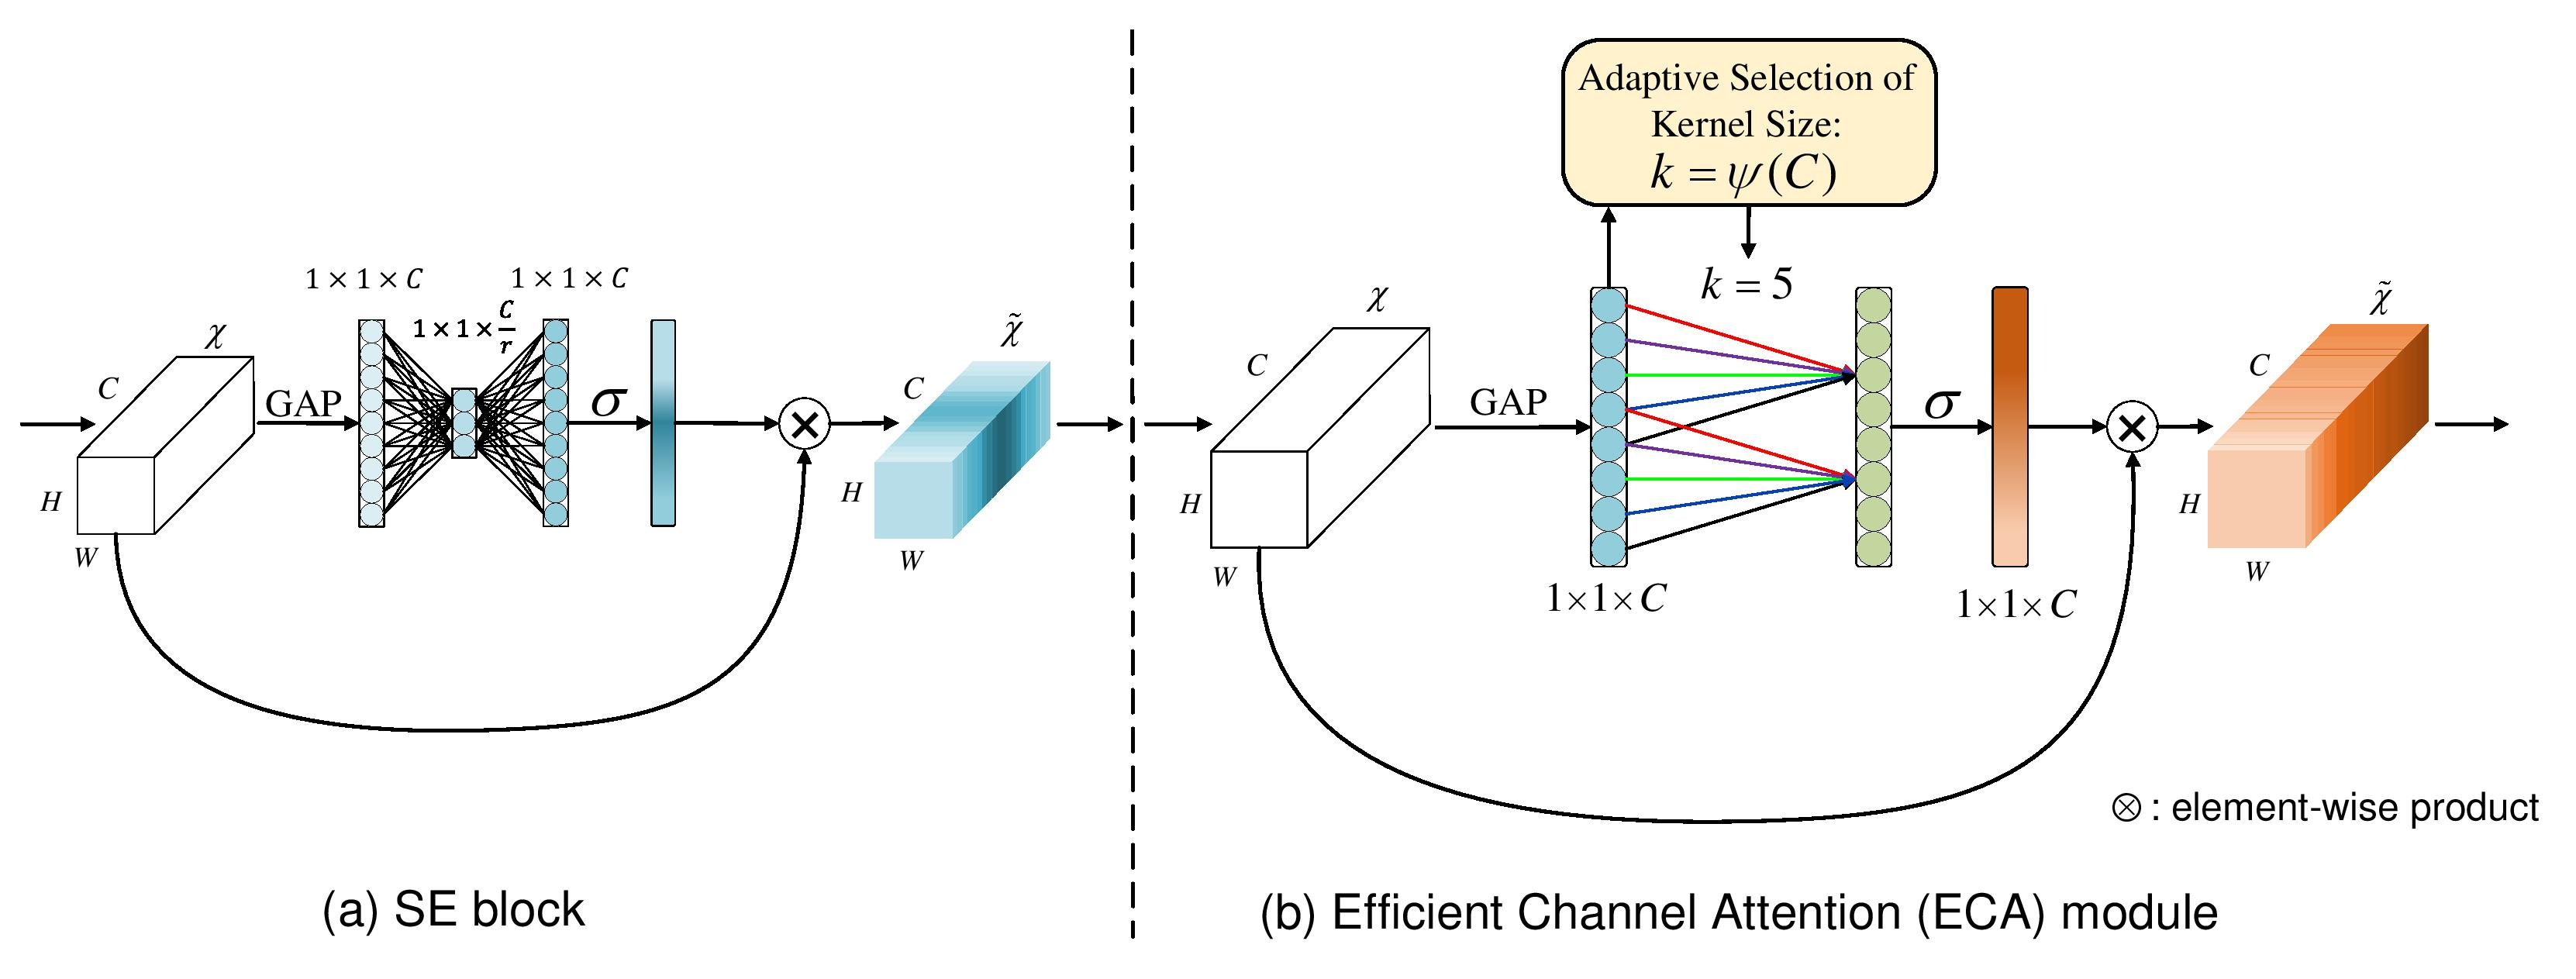
\includegraphics[width=1\textwidth]{images/eca_module.jpg}
\end{figure}


\subsection{Pre-Activation}
Pre-activation changes the order of activation and convolution inside default ResNet block, it makes training easier and improves generalization. It was introduced by authors of original ResNet50 model \cite{he2016deep_resnetv1} in their following paper \cite{he2016identity_resnetv2} but didn't become popular, despite noticeably better performance. 
The idea of pre-activation arose from attempts to train a very deep ResNets. The convergence speed and final performance of such models is degraded significantly with increasing depth which is contr-intuitive. A deeper net should be not worse than shallower net because it could be viewed as a shallow net with identity blocks stacked on top of it. But in reality the identity breaks because of activations in the main path of information. To recap an original ResNet block is shown on Figure \ref{fig: pre-act}. Given input of residual unit $x_l$ the output $x_{l+1}$ could be expressed in the following form: 
$$ x_{l+1} = ReLU \left( x_l + \mathcal{F} (x_l, W_l) \right)$$ \label{eq: res-block}

Where $\mathcal{F}$ calculates output of residual block which consists of Conv $\rightarrow$ BN $\rightarrow$ ReLU $\rightarrow$ Conv $\rightarrow$ BN. Where ReLU activation after addition has two undesired properties. First it breaks the propagation of identity signal which has been shown to be a crucial ingredient of success for residual networks \cite{chao2019_hardnet}. Secondly it limits all features in main path to positive values which introduces undesired constrains and limits model capacity. By rearranging blocks from $Conv \rightarrow BN \rightarrow Activation$ to $BN \rightarrow Activation \rightarrow Conv$ we can remove this properties while maintaining the same number of activations and convolution layers. Later in the paper we refer to such networks using pre-activation blocks as Pre-Activation ResNets.


% TODO: ideally - redraw this figure. or at least embed in correctly. 
% TODO: add plot for Linear Bottleneck which is the same as original block but without last ReLU
\begin{figure}[h!]
  \caption{ (a) original Residual Unit in [1]; (b) proposed Residual Unit}
  % The grey arrows indicate the easiest paths for the information to propagate, corresponding to the additive term “xl” in Eqn.(4) (forward propagation) and the additive term “1” in Eqn.(5) (backward propagation).
  \label{fig: pre-act}
  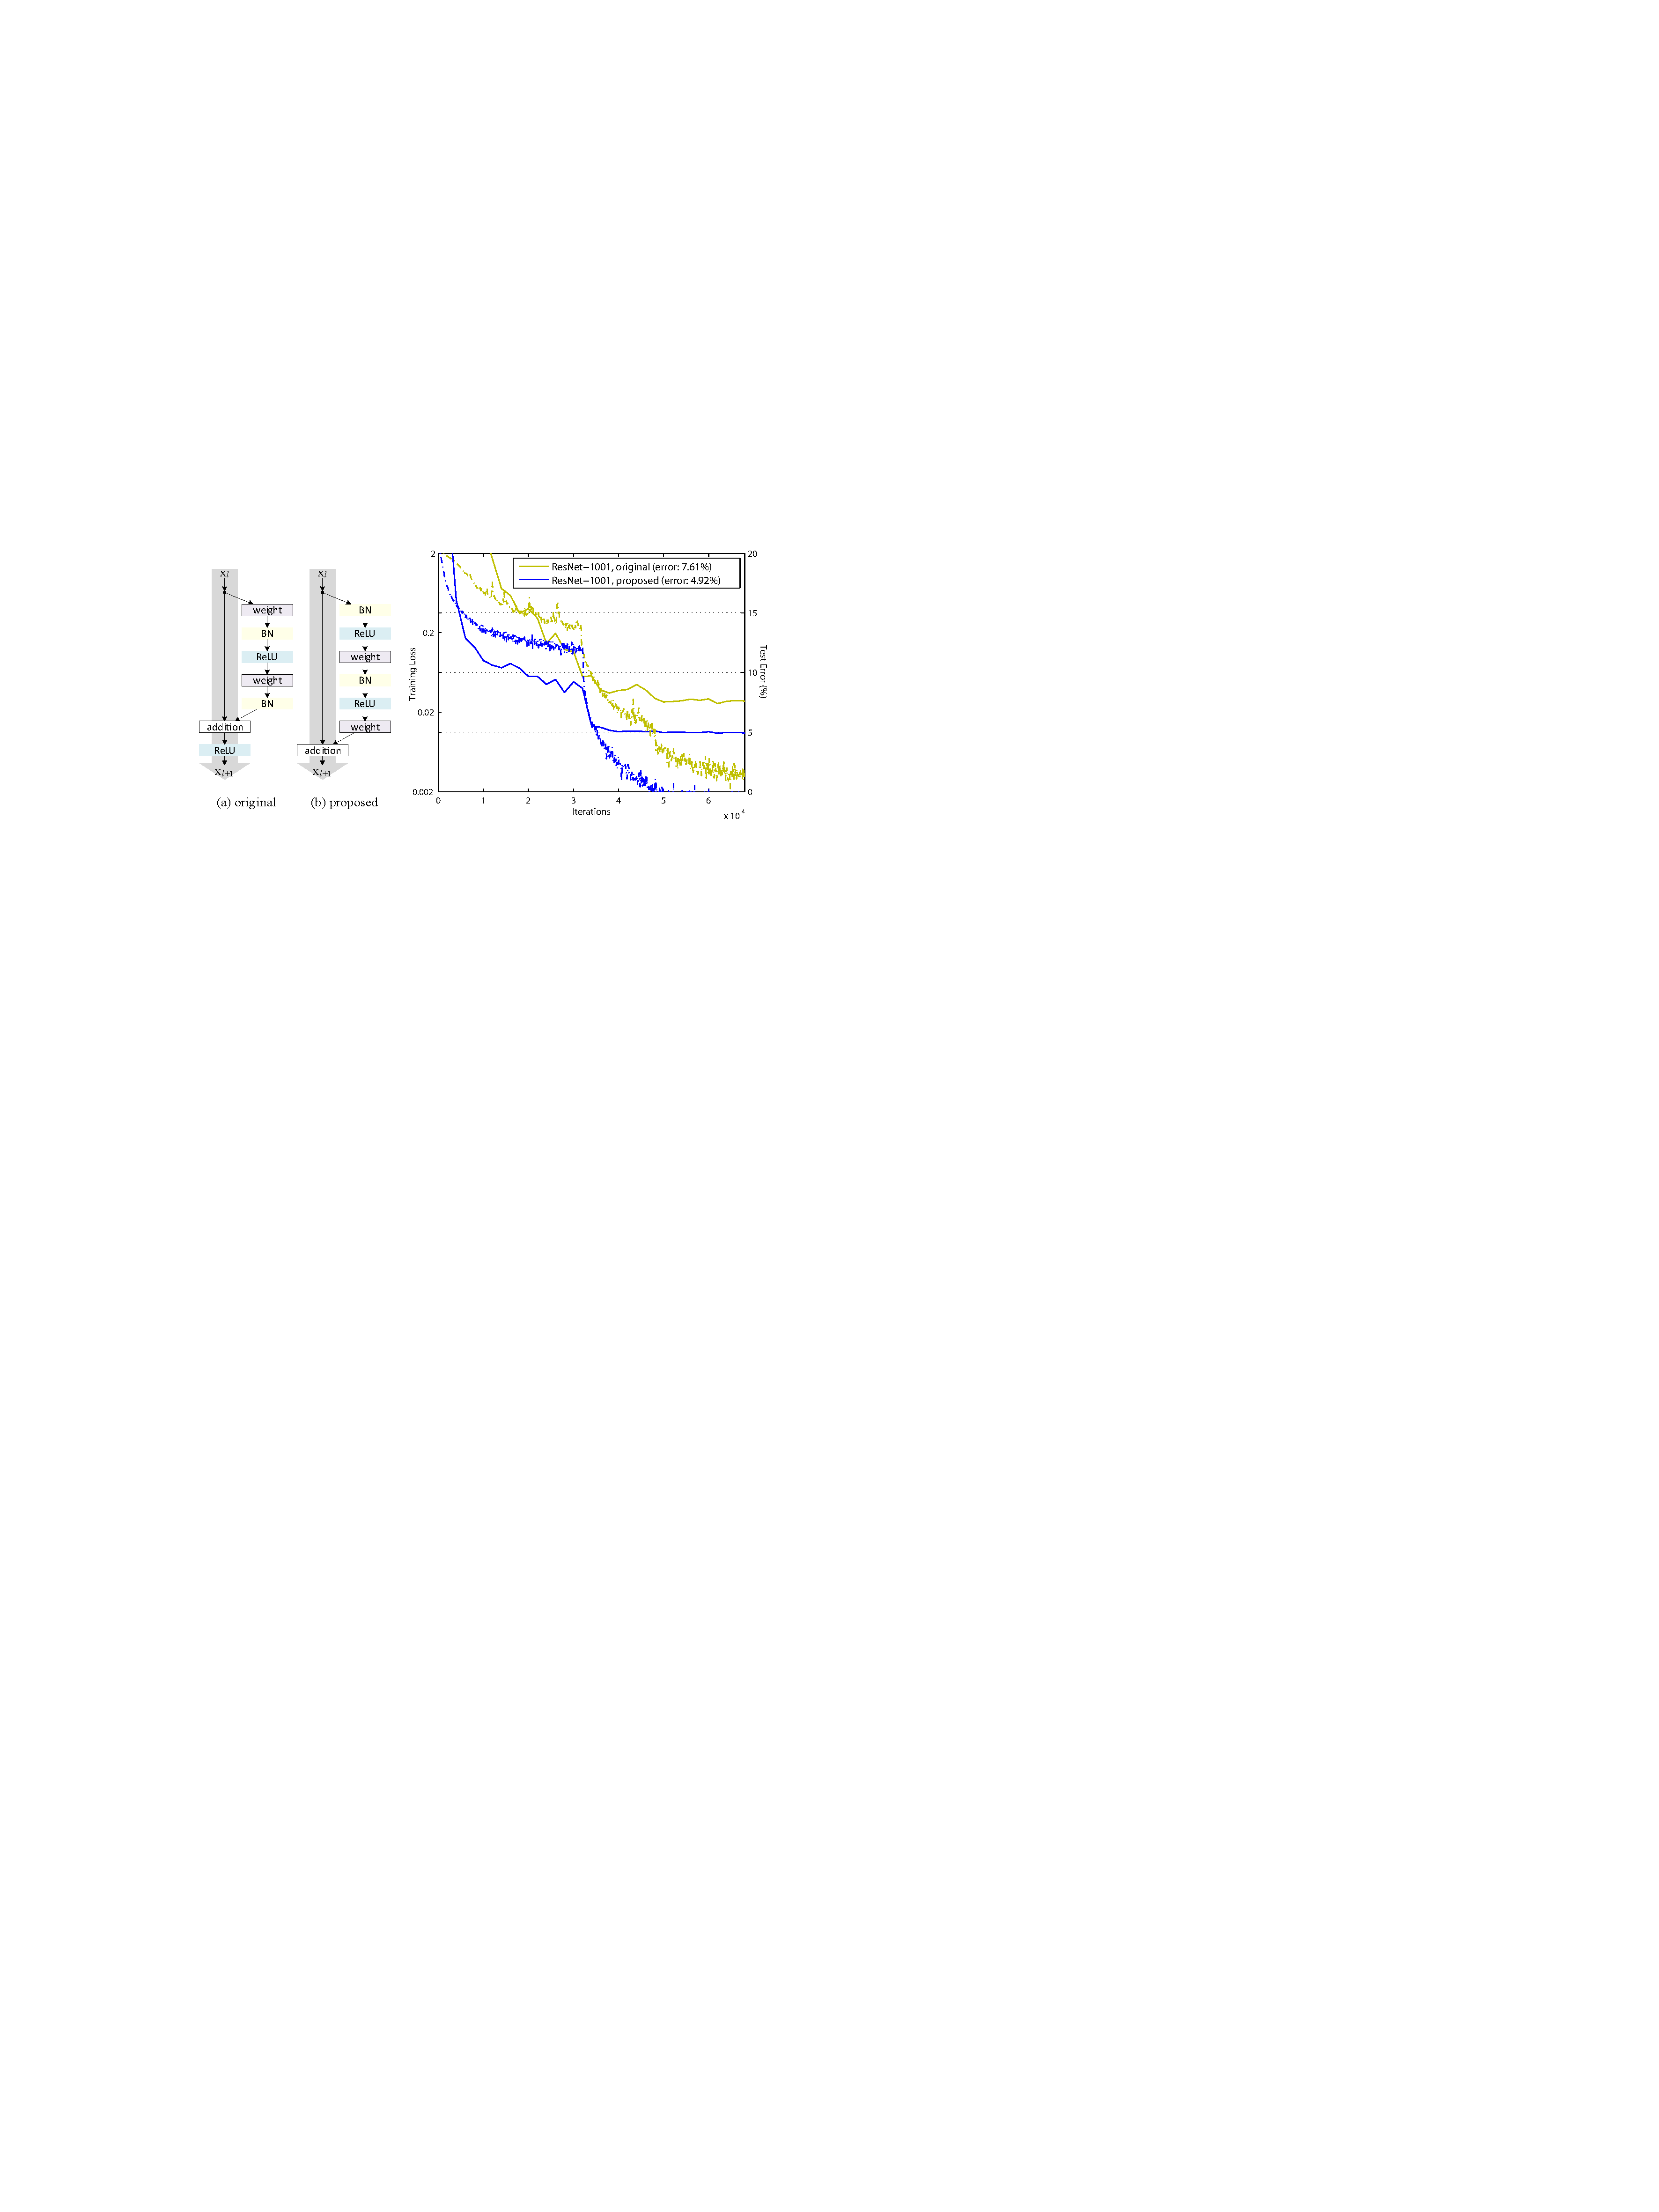
\includegraphics[clip, trim=0cm 0cm 13.5cm 0cm, scale=.55]{images/preact1.pdf}
\end{figure}

\subsection{Linear Bottleneck}
"Linear Bottleneck" \cite{sandler2018_mobilenetv2} tries to improve information propagation inside ResNet by removing the last ReLU activation from default block. The motivation for this is similar to Pre-Activation blocks - to prevent non-linearities from destroying too much information in the main path. We perform and ablation study between Pre-Activation and Linear Blocks later in Section \ref{sec:ablation}


% (когда буду говорить про SE vs ECA сделать ремарку о том, что авторы второго не правы, когда мерят ФЛОПс и говорят что у них меньше. может быть добавить эксперименты со скоростью если делать просто GAP без каких либо операций и показать что он занимает бОльшую часть от замедления (сколько это кстати? 60? 70?))
% upd. как оказалось, для большой картинки GAP занимает ~33% всего времени, для тензора в середине 25%, что составляет меньшую часть в любом случае. разница в скорости между ними определенно есть.  
% [ Middle stem. Shape: torch.Size([64, 32, 224, 224]) ]
%                      |  description
% 16 threads: -----------------------
%       GAP            |       7.7
%       SE(0.5). 1.1k  |      23.9
%       ECA            |      23.2
%       ECA9           |      23.2

% Times are in microseconds (us).

% [ Deeper stem. Shape: torch.Size([64, 256, 14, 14]) ]
%                       |  description
% 16 threads: ------------------------
%       GAP             |      352.0
%       SE(0.5). 33.1k  |     2491.0
%       ECA             |     1480.1
%       ECA9            |     1563.4

% Times are in nanoseconds (ns).



%% END OF SECTION

% The following section 
% Novel architectures are often simultaneously introduced with other critical – and less publicized – changes in the details of the training methodology and hyperparameters. Additionally, new architectures enhanced by modern training methods are sometimes compared to older architectures with dated training meth- ods (e.g. ResNet-50 with ImageNet Top-1 accuracy of 76.5\% \cite{he2016deep_resnetv2}. Our work addresses these issues and empirically studies the impact of training methods and scaling strategies on the popular ResNet architecture





%% 
% уже писал, но можно написать план еще раз. говорю, что новые статьи улучшаются и за счет блоков и за счёт улучшения тренировки, причем часто авторы статей не разделяют одно от другого, хочется посмотреть, на что способны старые архитектуры, если учить их новыми методами (это примерно то что пишут авторы резнет РС). в этой главе бОльшую часть нужно потратить на обзор маленьких улучшений, предложенных в последние годы (???)

%%
% нужно понять в каком порядке излагать мысль вообще. есть статьи, которые улучшают архитектуру, а есть которые предлагают новые способы обучения. проблема в том, что это не всегда разные статьи. новые блоки часто идут вместе с новыми трюками и сложно их разделить. (о чём пишут в compounding performance и гораздо более явно в resnet-RS). можно написать то же самое и сказать что "я был первым" что на самом деле так, я об этом еще в начале прошлого года разговаривал). но мне для диплома нужно много текста, поэтому надо как-то завернуть рассуждения. как завернуть? 

% разница между compounding и resnetRS в том, что первые бустят resnet без явного разделения что приходит от новых методов, а что приходит от изменения архитектуры, а RS явно показывает что приходит от архитектуры. 

%%





% at- tempts to combine existing techniques to create a practical model are still uncommon

% (нужно еще где-то сказать что со временем растет уровень того что такое бейзлайн. если в 2016м году резнет50 был 75.6, то сейчас если он ниже 79, то сравнение нечестное. самое честное что можно (и нужно делать) это использовать одинаковые трюки как во время обучения своей новой супер-пупер мега модели так и во время обучения старого-доброго резнета)



% \subsection{How to do better}



% (когда буду говорить про пайплайн, нужно вставить что дефолтные аугментации очень слабые и хотя это uncommon to report training accuracy for the model, one can observe a very strong overfitting using the default augmentation. it means that almost any additional regularization would have a noticeable effect, but it also means that что они бьют лежачего в общем    )


% The question is, when does ResNet50 stop being ResNet50? How many architecture changes is needed to be able to call it a new model? Why majority of people do not modify block structure, while making strong modifications of blocks themselves? The answer is probably because experiments on ImageNet are quite expensive and not everyone has resources and time and knowledge to explore all possible variations. This is where papers like mine come into place with thorough examination of already proposed techniques and how do they combine together

% когда буду говорить про переход к ResNet D нужно не просто представить новую архитектуру, а попытаться объяснить какие именно проблемы она решает. типа страйд не там или что




% (тут ли?)
% Говорю о том что в последнее время появилось много маленьких улучшений, которые не замедляют сеть, но дают буст по качеству \cite{zhang2019making_aa_shift_invariant} или space2depth  \cite{ridnik2021_tresnet} в начале сети. были статья которые объединяли это все вместе \cite{lee2020compounding_improvements} \cite{bello2021revisiting_resnet} (ну и как бы мои результаты не лучше чем у них, просто они тупо стакают все изменения на резнет, а я еще и архитектуру меняю после этого, чтобы учесть архитектурные недостатки


% говно разбиение на главы. чем глава 3 отличается от главы 4?
% в 3.1 говорю про улучшения тренировочного пайплайна, в 3.2 про улучшения архитектуры? 
% но нужно как-то подвести к этому, а не тупо начинать вываливать на читателей списки новых слоёв??


% Глава2 - про скорость и связь со флопсами и все такое
% Глава3 - про улучшения обучения связанные с ванильным R50
% Глава4 - про связку небольших изменений и медленные изменения архитектуры опираясь на то, что работает у других
% Глава5 - design choice not present in current literature

